\begin{figure}[h!]
    \centering
    \caption{Counterfactual increases in residence and workplace MWs at urban ZIP
    	codes of raising the federal MW to \$9 in January 2020}
    \label{fig:cf_res_and_wkp_changes}
	\begin{subfigure}{0.51\textwidth}
		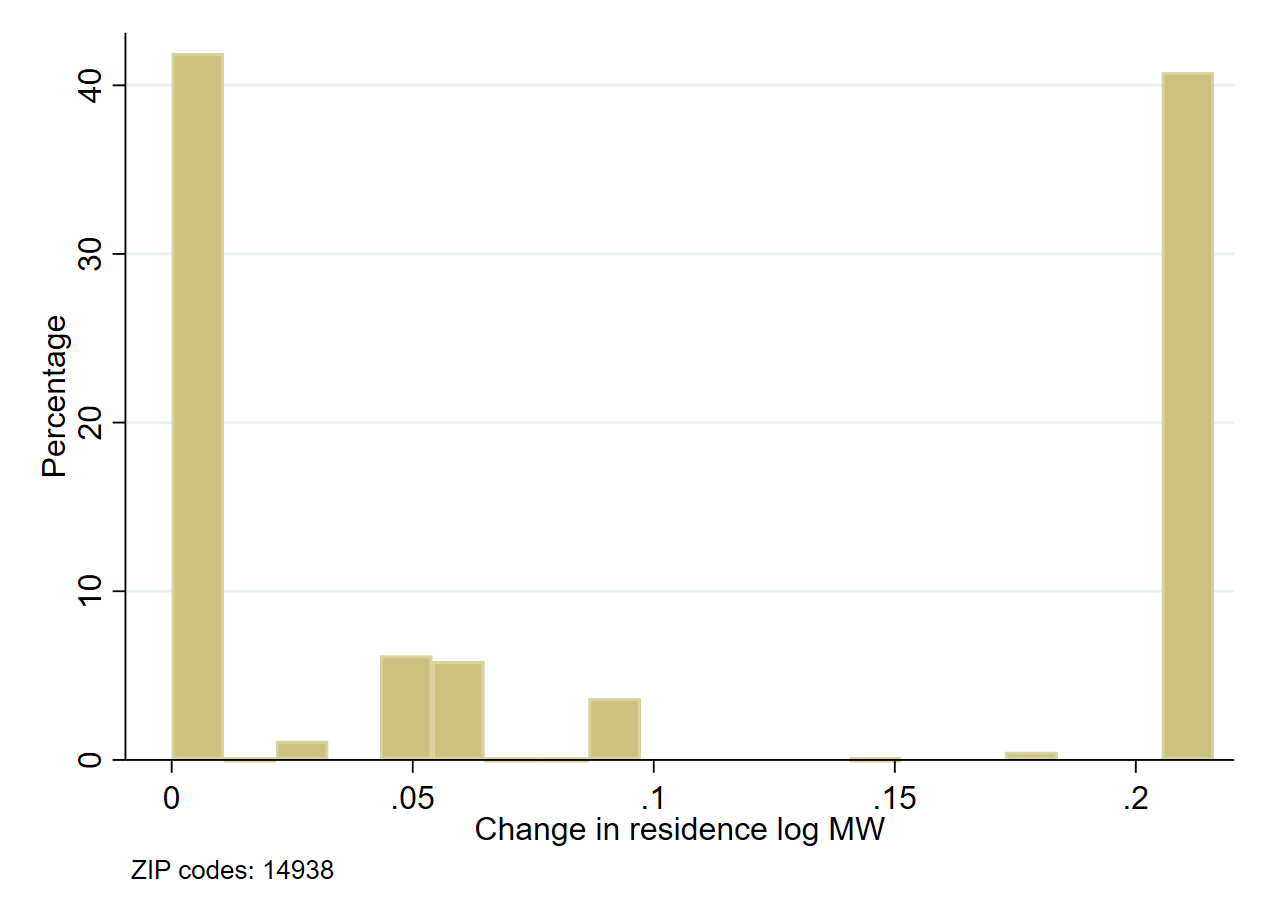
\includegraphics[width = 0.99\textwidth]{counterfactuals/output/d_mw_res.png}
		\caption*{Residence MW}
	\end{subfigure}%
	\begin{subfigure}{0.51\textwidth}
		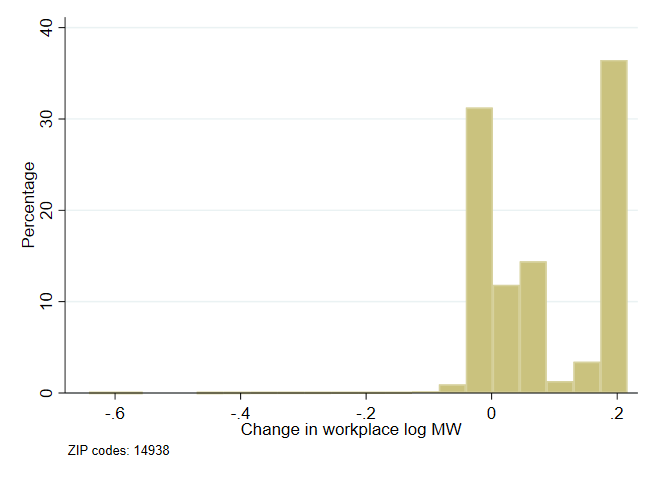
\includegraphics[width = 0.99\textwidth]{counterfactuals/output/d_mw_wkp_tot_17.png}
		\caption*{Workplace MW}
	\end{subfigure}

\begin{minipage}{.95\textwidth} \footnotesize
	\vspace{3mm}
	Notes: 
	The unit of observation is a ZIP code. We code a ZIP code as urban if it 
	has at least 20\% of its population being urban.
	Changes are computed as explained in Section \ref{sec:cf_res_and_wkp_changes}.
	Panel (a) displays counterfactual changes for the residence MW measure.
	Panel (b) displays counterfactual changes for the workplace MW measure.
\end{minipage}
\end{figure}